\documentclass[12pt]{article}
\usepackage[utf8]{inputenc}
\usepackage[spanish]{babel}
\usepackage{amsmath, amssymb, amsthm}
\usepackage{graphicx}
\usepackage{float}
\usepackage{hyperref}
\usepackage{geometry}
\geometry{a4paper, margin=1in}

\title{Proyecto MAT-043: Probabilidad y Estadística}
\author{Francisco Gonzalez, Karime Jarufe\\ Universidad Técnica Federico Santa María}
\date{Noviembre 25, 2024}

\begin{document}

\maketitle

\tableofcontents
\newpage

\section{Introducción}
Este proyecto aborda distintos problemas relacionados con la probabilidad y estadística aplicadas, empleando herramientas computacionales y métodos de simulación Monte Carlo. El objetivo principal es aplicar conceptos teóricos a situaciones prácticas y obtener resultados analíticos y simulados.

\section{Metodología}
\subsection{Herramientas Utilizadas}
Describa las herramientas computacionales (por ejemplo, Python, R, MATLAB, etc.) y bibliotecas usadas para la resolución de problemas. También explique brevemente los métodos teóricos relevantes, como histogramas, simulación Monte Carlo, o transformaciones de variables aleatorias.

\subsection{Estructura del Proyecto}
El proyecto se divide en los siguientes problemas, cada uno abordado de manera independiente con análisis teórico y computacional:
\begin{itemize}
    \item Problema 1: Análisis de precios de casas en Ames, Iowa.
    \item Problema 2: Estimación de asientos extra en vuelos.
    \item Problema 3: Probabilidad de atención en un peaje.
    \item Problema 4: Simulación de capacidad en una sala de operaciones.
    \item Problema 5: Distancia esperada entre dos distribuciones normales.
\end{itemize}

\newpage

\section{Desarrollo}
\subsection{Problema 1: Análisis de Precios de Casas}
En este problema se analiza la variable \textit{SalePrice} del conjunto de datos \textit{Ames Housing}. Este análisis incluye la visualización de datos mediante gráficos, el ajuste de una distribución de densidad, y el cálculo de probabilidades y valores esperados.

\subsubsection{Análisis Descriptivo}
Se construyeron los siguientes gráficos para la variable \textit{SalePrice}:
\begin{enumerate}
    \item Un histograma para observar la distribución de frecuencias.
    \item Un boxplot y un violin plot para visualizar la dispersión y detectar posibles valores atípicos.
\end{enumerate}

Los gráficos generados se presentan en las figuras \ref{fig:histograma} y \ref{fig:boxplot_violin}.

\begin{figure}[H]
    \centering
    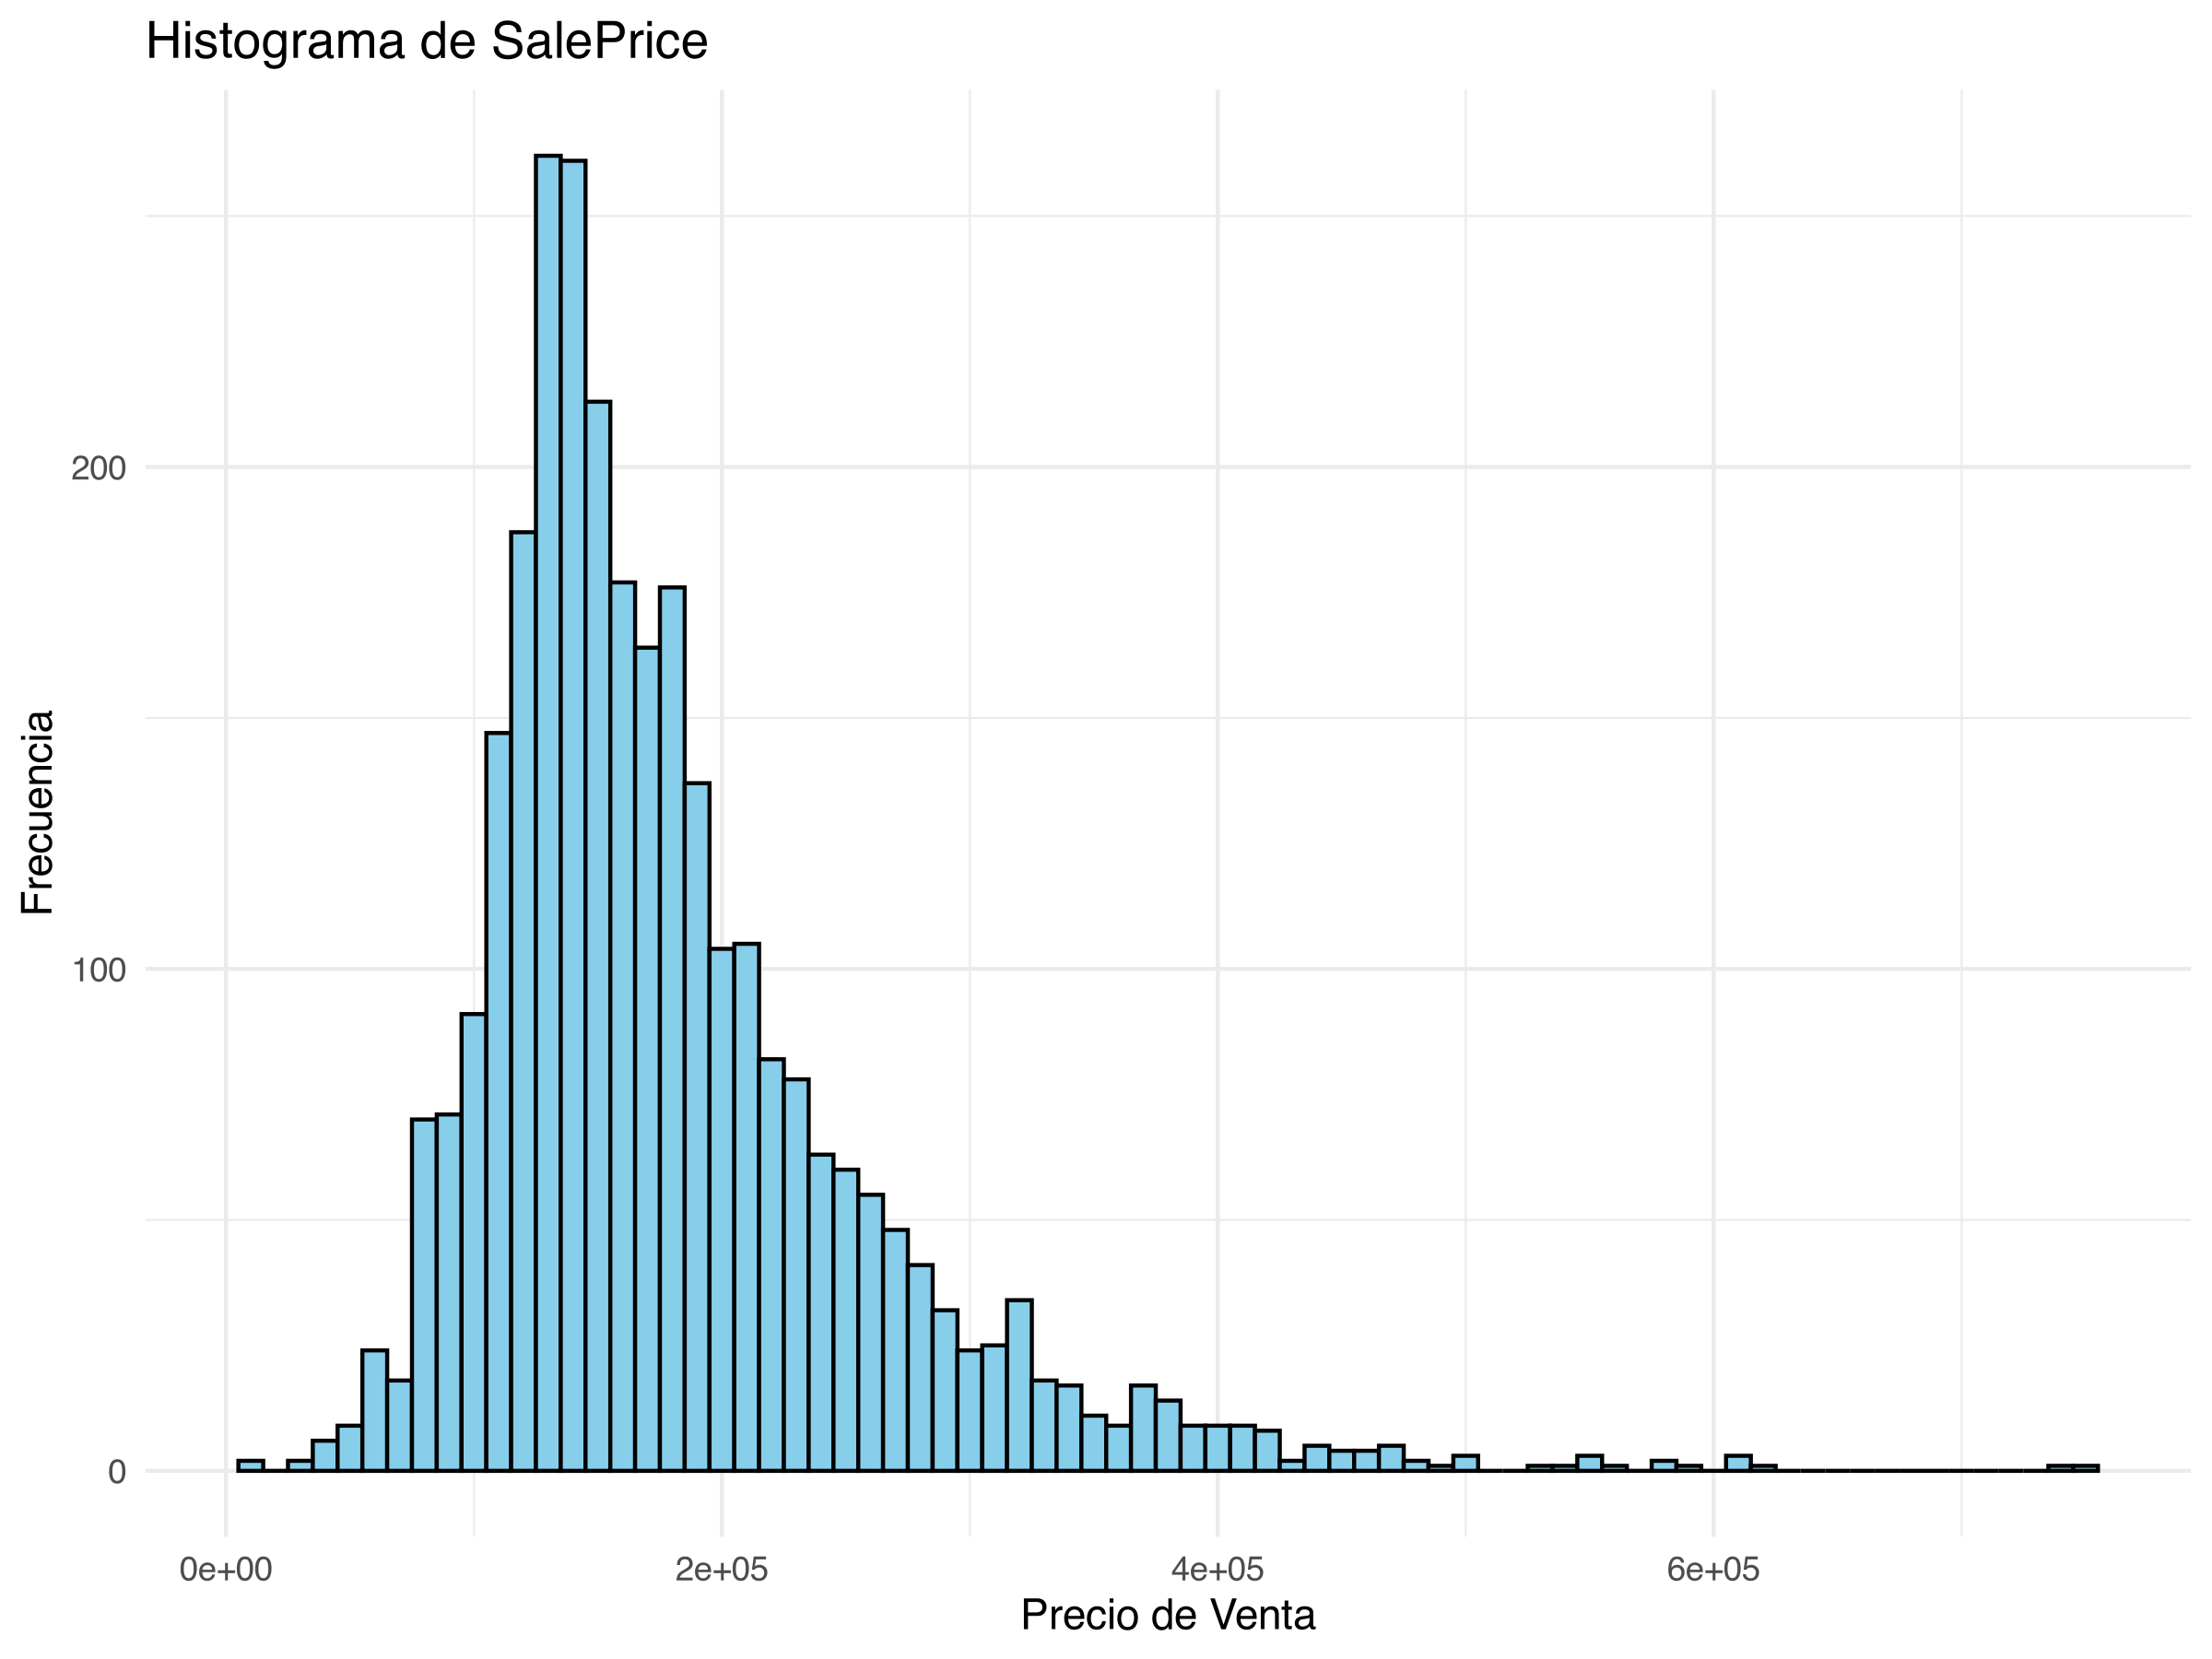
\includegraphics[width=0.8\textwidth]{histograma_saleprice.png}
    \caption{Histograma de la variable \textit{SalePrice}.}
    \label{fig:histograma}
\end{figure}

\begin{figure}[H]
    \centering
    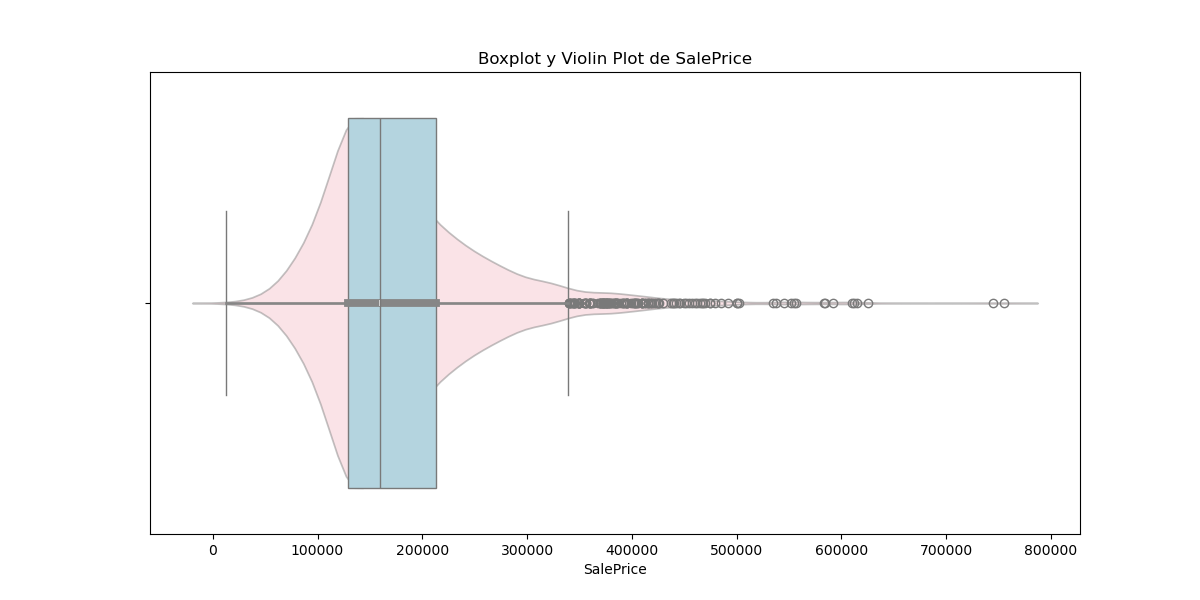
\includegraphics[width=0.8\textwidth]{boxplot_violin_saleprice.png}
    \caption{Boxplot y violin plot de la variable \textit{SalePrice}.}
    \label{fig:boxplot_violin}
\end{figure}

\subsubsection{Ajuste de una Distribución de Densidad}
El análisis del histograma sugiere que los datos de \textit{SalePrice} presentan asimetría positiva. Se ajustó una distribución log-normal utilizando el método de máxima verosimilitud. La función de densidad ajustada es:

\[
f(x) = \frac{1}{x \sigma \sqrt{2\pi}} e^{-\frac{(\ln x - \mu)^2}{2\sigma^2}}, \quad x > 0.
\]

Los parámetros estimados fueron:
\begin{itemize}
    \item Media logarítmica ($\mu$): XXX
    \item Desviación estándar logarítmica ($\sigma$): XXX
\end{itemize}

\subsubsection{Cálculo de Probabilidades y Valor Esperado}
Con base en la distribución ajustada:
\begin{enumerate}
    \item La probabilidad de que una casa cueste más de 200,000 USD es:
    \[
    P(X > 200,000) = 1 - F(200,000),
    \]
    donde $F(x)$ es la función de distribución acumulada.
    \item El valor esperado del precio de las casas es:
    \[
    E[X] = e^{\mu + \sigma^2 / 2}.
    \]
\end{enumerate}

Los resultados obtenidos fueron:
\begin{itemize}
    \item Probabilidad: XXX
    \item Valor esperado: XXX
\end{itemize}


\subsection{Problema 2: Estimación de Asientos Extra en Vuelos}
\begin{enumerate}
    \item Explicación del modelo de Poisson y simulación Monte Carlo.
    \item Resultados de simulación para los tres tipos de aviones.
\end{enumerate}

\subsection{Problema 3: Probabilidad de Atención en un Peaje}
\begin{enumerate}
    \item Uso de distribuciones normales y exponenciales para modelar la cantidad de autos atendidos.
    \item Implementación del algoritmo de simulación.
\end{enumerate}

\subsection{Problema 4: Capacidad de una Sala de Operaciones}
\begin{enumerate}
    \item Modelado de tiempos usando distribuciones normales, exponenciales y uniformes.
    \item Simulación de la cantidad de pacientes atendidos en un mes.
\end{enumerate}

\subsection{Problema 5: Distancia entre Distribuciones Normales}
\begin{enumerate}
    \item Aplicación de propiedades de distribuciones normales para calcular $E[|X - Y|]$.
\end{enumerate}

\newpage

\section{Resultados}
\subsection{Gráficos y Tablas}
Incluya aquí todos los gráficos generados (histogramas, boxplots, etc.) y las tablas de resultados relevantes para cada problema.

\subsection{Análisis de Resultados}
Discuta los patrones observados en los datos, la precisión de los modelos ajustados y cualquier hallazgo relevante de las simulaciones.

\section{Conclusiones}
Resuma los principales hallazgos del proyecto y reflexione sobre la aplicabilidad de los métodos empleados en problemas reales.

\section{Apéndices}
\subsection{Código Fuente}
Incluya el código fuente utilizado para resolver los problemas.

\subsection{Referencias}
Proporcione referencias a artículos, libros, o recursos en línea utilizados.

\end{document}
